\documentclass[numbering=fraction]{beamer}

\usepackage[utf8]{inputenc}
\usepackage[T1]{fontenc}
\usepackage[french]{babel}
\usepackage{blindtext}
\usepackage{tikzsymbols}
\usepackage{graphicx}
\usepackage{wrapfig}
\usepackage{bookman}
\usepackage{subcaption}
\usepackage[export]{adjustbox}



\usetheme[progressbar=frametitle]{metropolis}

%Define colors
\definecolor{wuppergreen}{RGB}{85, 171, 38}
\definecolor{background}{RGB}{255,255,255}

%Adding logo to title page
\titlegraphic{\raggedleft 
\includegraphics[width=3cm]{UNamur.png}}

%Adjust color theme
\setbeamercolor{frametitle}{bg=wuppergreen}
\setbeamercolor{title separator}{fg=wuppergreen}
\setbeamercolor{footline}{fg=gray}
\setbeamercolor{progress bar}{fg=black}

%Adding footer
\setbeamertemplate{frame footer}{\insertshortauthor~(\insertshortinstitute)}

\graphicspath{ {../Images/}}

%Set parameters for title page
\title{PIMS : Sprint Review 3}
\author[PIMS]{Luis Dierick \and Gaillard Matthys \and Bouncer Yassine \and Fundu Oliver \and Anderson Rosny \and Tom Marchal }
\institute{Université de Namur}
\date{\today}

\begin{document}

\begin{frame}[plain]{}
    \maketitle
\end{frame}

\begin{frame}{Table des matières}
    \tableofcontents
\end{frame}
\section{Base de données}
\begin{frame}{Base de données}
    \begin{enumerate}
        \item Impléntée avec PostGreSQL
        \item Dispose de divers avantages
        \begin{itemize}
            \item Sécurité : Niveau de protection élevé (2 couches supplémentaires)
            \item Large choix de type de données diverses : texte, document, JSON, autre, \dots
            \item Rapidité : Permet de gérer de grandes quantités de données grâce à son architecture permettant des bases de données distribuées
        \end{itemize}
    \end{enumerate}
\end{frame}
\subsection{Schéma de la base de données}
\subsubsection{Schéma de la base de données - schéma relationnel}
\begin{frame}{Schéma de la base de données}
    \begin{figure}
        \centering
        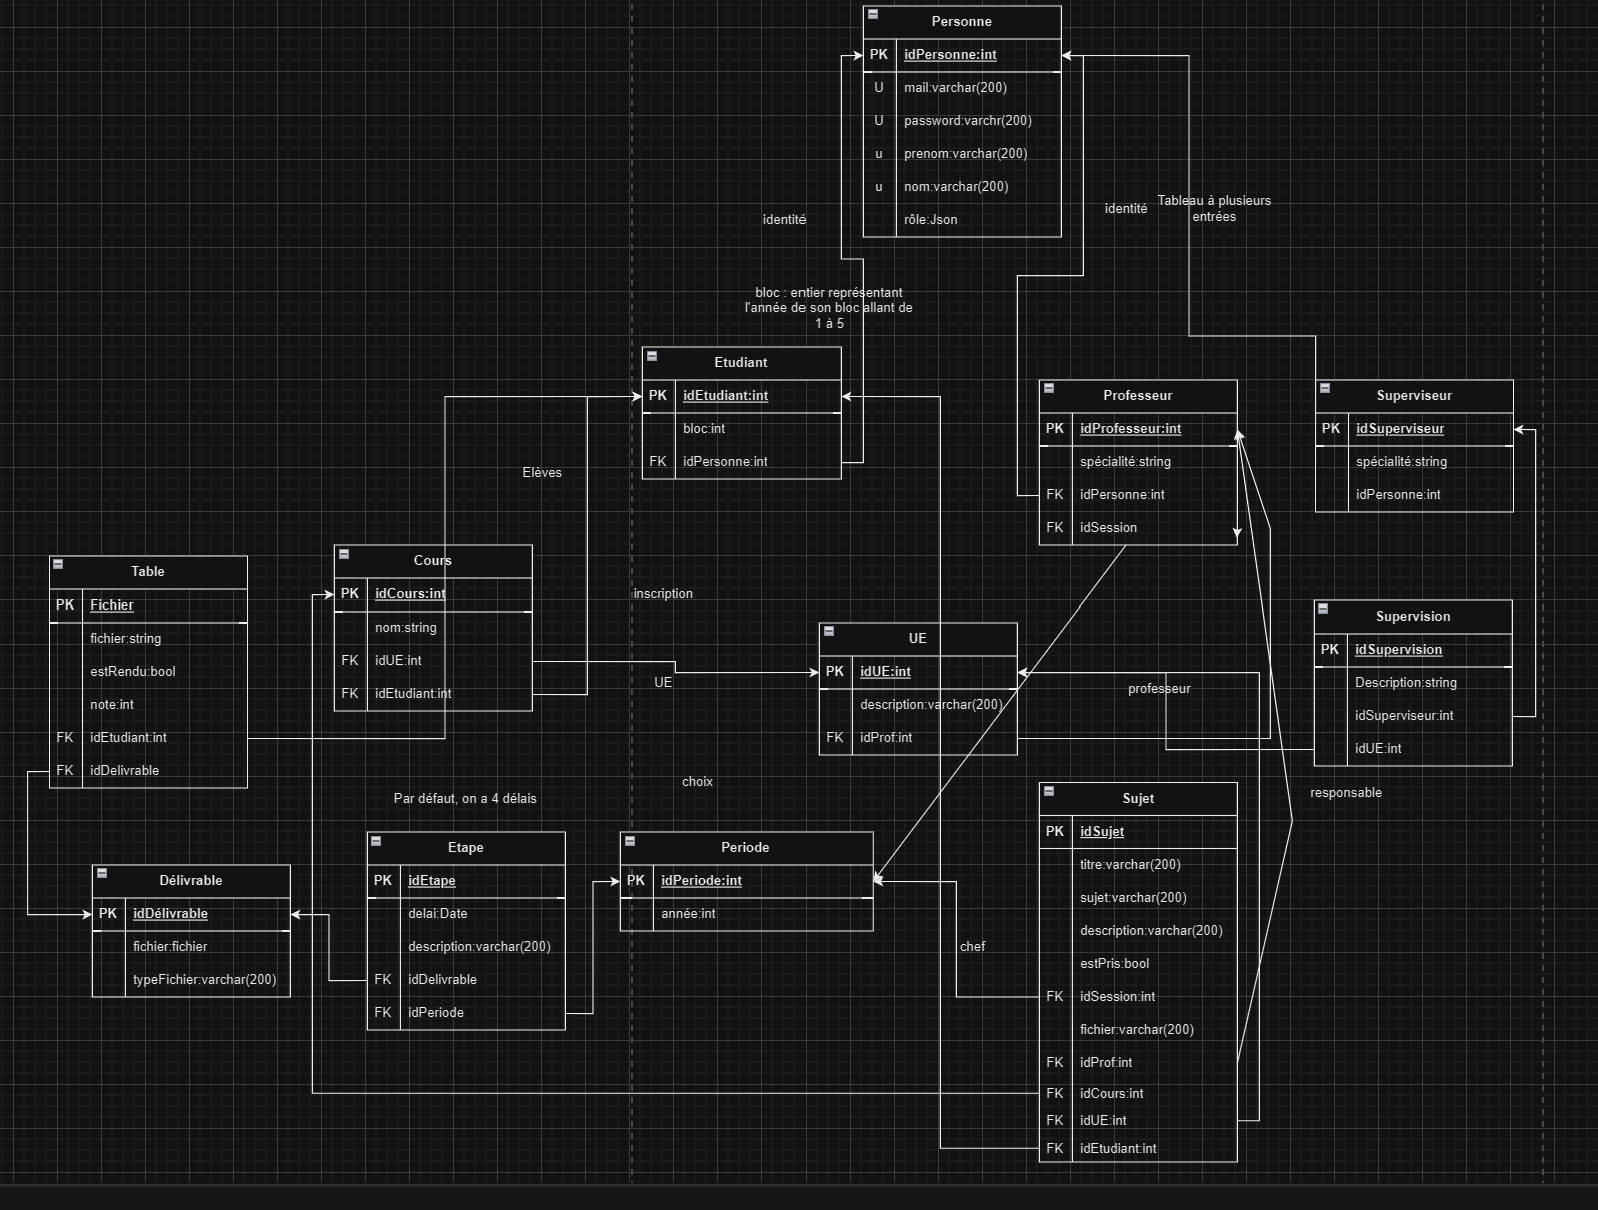
\includegraphics[width=0.8\textwidth]{dbrelation.png}
        \caption{Schéma de la base de données}
    \end{figure}
\end{frame}
\subsubsection{Schéma de la base de données - schéma entité-relation}
\begin{frame}{Schéma de la base de données- schéma entité-relation}
    \begin{figure}
        \centering
        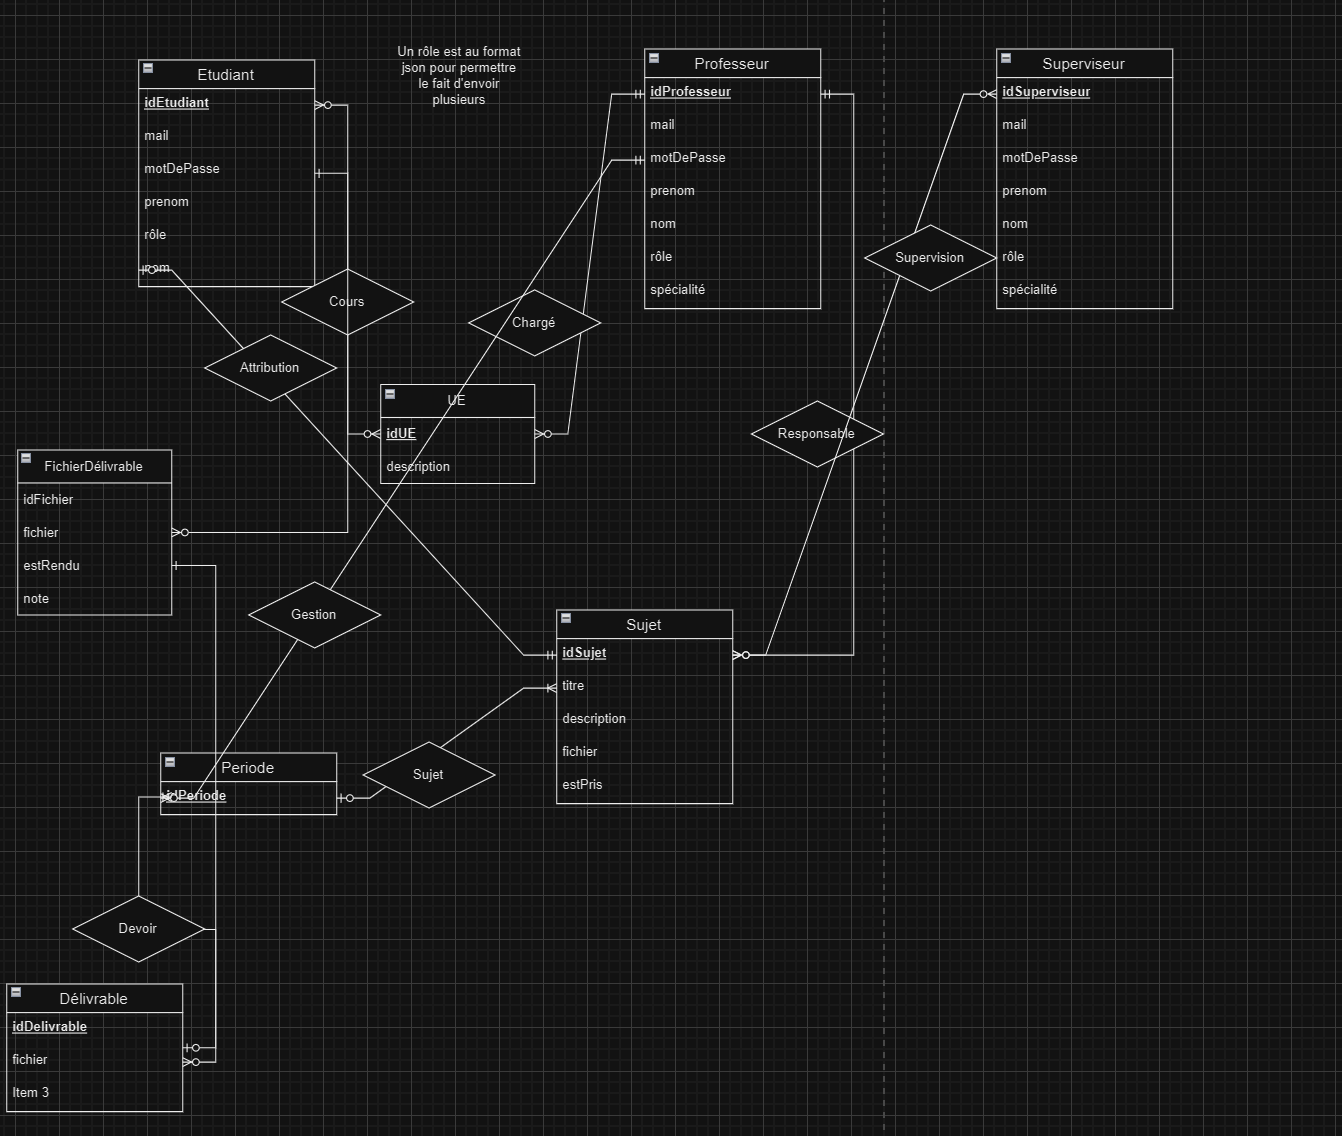
\includegraphics[width=0.8\textwidth]{dbER.png}
        \caption{Schéma de la base de données}
    \end{figure}
\end{frame}
\end{document}  